\documentclass{standalone}

\usepackage[siunitx,americanvoltages, europeanresistors,americancurrents]{circuitikz}
\usepackage{color}
\usepackage{graphicx}%Für Grafiken
\usepackage{rotating} % lässt Grafiken rotieren
\usepackage{mathtools}% mathematische Werkzeuge
\usepackage{amsmath}% Mathetools
\usepackage{amsfonts}% Mathetools
\usepackage{physics}
\usepackage{amssymb}% Symbole wie Natürliche Zahlen
\usepackage{geometry}
\usepackage{caption} % Unter-/Überschriften für Bilder, Grafiken und Tabellen
\usepackage{tikz}
\usepackage{amsthm}

% tikz libraries
\usetikzlibrary{arrows}
\usetikzlibrary{3d}
\usetikzlibrary{angles, quotes, shapes, decorations.markings, calc, arrows.meta}

% mathmatical commands
\newcommand{\AAA}{\mathbf{A}}
\newcommand{\R}{\mathbb{R}}
\newcommand{\N}{\mathbb{N}}
\newcommand{\p}{\mathcal{P}}
\newcommand{\I}{\infty}
\newcommand{\ve}{\varepsilon}
\newcommand{\vp}{\varphi}

\begin{document}
	
	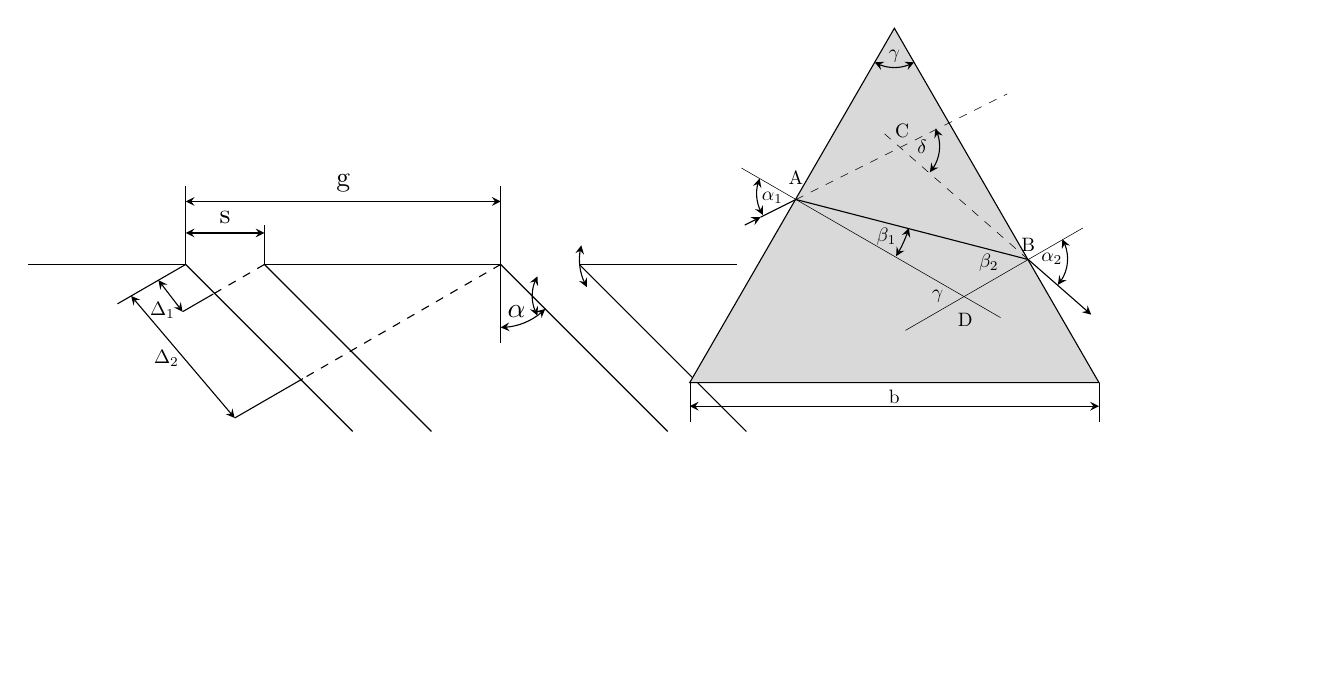
\begin{tikzpicture}[>=stealth]
		\draw[white] (-6,-5) rectangle (10,1);
		\draw (-6,0) -- (-4,0);
		\draw (-3,0) -- (0,0);
		\draw (1,0) -- (3,0);
		\draw (-4,0) -- ({-4+cos(315)*3},{sin(315)*3});
		\draw (-3,0) -- ({-3+cos(315)*3},{sin(315)*3});
		\draw (0,0) -- ({cos(315)*3},{sin(315)*3});
		\draw (1,0) -- ({1+cos(315)*3},{sin(315)*3});
		\draw (-4,0) -- (-4,1);
		\draw (-3,0) -- (-3,.5);
		\draw (0,-1) -- (0,1);
		
		% Linien
		\draw (-4,0) -- ({-4+cos(210)*1},{sin(210)*1});
		\draw[dashed] (-3,0) -- ({-3+cos(210)* .8},{sin(210)* .8});
		\draw[dashed] (0,0) -- ({cos(210)*2.9},{sin(210)*2.9});
		\draw ({cos(210)*2.9},{sin(210)*2.9}) -- ({cos(210)*3.9},{sin(210)*3.9});
		\draw ({-3+cos(210)*.75},{sin(210)*.75}) -- ({-3+cos(210)*1.2},{sin(210)*1.2});
		
		% Pfeile und Bezeichnungen
		\draw[<->] (-4,.8) -- (0,.8);
		\node[above] at (-2,.8) {g};
		\draw[<->] (-4,.4) -- (-3,.4);
		\node[above] at (-3.5,.4) {s};
		\draw[<->] (0,-.8) arc (270:315:.8);
		\node at (.2,-.6) {$\alpha$};
		\draw[<->] ({-4+cos(210)*.8},{sin(210)*.8}) -- ({cos(210)*3.9},{sin(210)*3.9});
		\draw[<->] ({-4+cos(210)*.4},{sin(210)*.4}) -- ({-3+cos(210)* 1.2},{sin(210)* 1.2});
		\node[scale=.7,below left] at (-4.05,-.395) {$\Delta_1$};
		\node[scale=.7,below left] at (-4.,-1) {$\Delta_2$};
		
		% Dreieck
		% Gleichwinkeliges Dreieck/Prisma
		\filldraw[fill=gray!30!white,draw=black] ({cos(90)*3+5},{sin(90)*3}) -- ({cos(210)*3+5},{sin(210)*3}) -- ({cos(330)*3+5},{sin(330)*3}) -- cycle;
		\draw[very thin] ({cos(210)*3+5},{sin(210)*3}) -- ({cos(210)*3+5},{sin(210)*3-.5});
		\draw[very thin] ({cos(330)*3+5},{sin(330)*3}) -- ({cos(330)*3+5},{sin(330)*3-.5});
		\draw[<->] ({cos(330)*3+5},{sin(330)*3-.3}) -- ({cos(210)*3+5},{sin(210)*3-.3});
		
		% Lichtstrahl und Geraden
		\draw[->] ({-1.9+5},0.5) -- ({-1.7+5},0.6);
		\draw[->] ({-1.7+5},0.6) -- ({-1.25+5},0.825) -- (6.7,.0625) -- (7.5,-0.6375);
		\draw[very thin]  ({-1.25+cos(60+90)*0.8+5},{0.825+sin(60+90)*0.8}) -- ({-1.25+5},0.825) -- ({-1.25+cos(-30)*3+5},{0.825+sin(-30)*3});
		\draw[very thin] ({1.7+cos(30)*0.8+5},{.0625+sin(30)*0.8}) -- ({1.7+cos(210)*1.8+5},{.0625+sin(210)*1.8});
		\draw[very thin,dashed] (6.7,.0625) -- ({6.7+cos(-41.1859+180)*2.5},{.0625+sin(-41.1859+180)*2.5});
		\draw[very thin,dashed] ({-1.25+5},0.825) -- ({-1.25+cos(26.5651)*3+5},{0.825+sin(26.5651)*3});
		
		% Punkte
		\node[scale=.7] at ({-1.25+5},1.1) {A};
		\node[scale=.7] at (6.7,.25) {B};
		\node[scale=.7] at (5.1,1.7) {C};
		\node[scale=.7] at (5.9,-0.7) {D};
		% Winkel
		\draw[<->] ({cos(300)*0.5+5},{sin(300)*0.5+3}) 
		arc (300:240:0.5);
		\node[scale=0.7] at (5,2.65) {$\gamma$};
		\draw[<->] ({-1.25+cos(157.5)*0.5+5},{.9+sin(157.5)*0.5}) arc (157.5:213:0.5);
		\node[scale=.7] at ({-1.55+5},.85) {$ \alpha_1 $};
		\draw[<->] ({0.075+cos(26.5651)*0.5+5},{1.5+sin(26.5651)*0.5}) arc (26.5651:-41.1859:0.5);
		\node[scale=.7] at (5.35,1.5) {$\delta$};
		\draw[<->] ({-1.25+cos(-17)*1.5+5},{sin(-17)*1.5+.9}) arc (-17:-32:1.5);
		\node[scale=.7] at (4.9,0.35) {$\beta_1$};
		\draw[<->] ({1.7+cos(210)*.7},{.0625+sin(210)*.7}) arc (210:165:.7);
		\node[scale=.7] at (6.2,0.025) {$\beta_2$};
		\draw[<->] ({.9+cos(210)*.5},{-.4+sin(210)*.5}) arc (210:150:.5);
		\node[scale=.7] at (5.55,-.4) {$\gamma$};
		\draw[<->] ({1.7+cos(210-180)*.5+5},{.07+sin(30)*.5}) arc (30:-41.1859:.5);
		\node[scale=.7] at (7,0.07) {$\alpha_2$};
		\node[above,scale=.7] at (5,{-1.857}) {b};
	\end{tikzpicture}
	
\end{document}
